\subsection{DNN Framework and Mining Methodology}

As a backbone, we employ ResNet-34 architecture \cite{resnet}.
We preserve the last dense feature layer in the ResNet-34 DNN
and remove the last flatten feature in the forward method and linear layer that is popularly used for image classification tasks.
The backbone downsamples the RGB image $I_{RGB} \in \mathbb{R}^{H \times W \times 3}$
to dense features $I_d \in \mathbb{R}^{h \times w \times D}$
such that $ h \ll H, w \ll W \text{ and } D \in \mathbb{N}^+$.
We directly upsample the dense features from the identity layer as illustrated in the Figure~\ref{fig:modified_dnn} in page~\pageref{fig:modified_dnn} as follows:
\begin{equation}
    f_U: I \in \mathbb{R}^{h \times w \times D} \rightarrow I_D \in \mathbb{R}^{H \times W \times D},
\end{equation}
the upsampled dense features substitutes as dense visual local descriptors produced from the DON.
Similarly as in \cite{suwajanakorn2018discovery}, we stack spatial-probability regressing layer and
depth regressing layer on top of the identity layer to predict $N \in \mathbb{N}^+$ number of keypoint's spatial-probability as follows:
\begin{equation}
    f_S: I_d \in \mathbb{R}^{h \times w \times D} \rightarrow I_s^N \in \mathbb{R}^{h \times w \times N} \text{ , such that } \sum^{h} \sum^{w} I_s^N = 1.0^N,
\end{equation}
and depth as follows:
\begin{equation}
    f_D: I_d \in \mathbb{R}^{h \times w \times D} \rightarrow I_{\hat{d}} \in \mathbb{R}^{h \times w \times N}.
\end{equation}

We incorporate continuous sampling method $f_E$ from \parencites{florence2020dense}{suwajanakorn2018discovery}
to convert the upsampled predicted spatial-probability and depth of a keypoint to spatial-depth expectation as follows:
\begin{equation}
    f_E \circ g_E:[I_s, I_{\hat{d}}] \rightarrow [u, v, d]^T \in \mathbb{R}^3 \text{ , where }  g_E: I \in \mathbb{R}^{h \times w \times N} \rightarrow I \in \mathbb{R}^{H \times W \times N}.
\end{equation}
Furthermore, we train the DNN in a twin architecture fashion as depicted in the Figure~\ref{fig:twin_architecture}
in page~\pageref{fig:twin_architecture} as proposed in
\parencites{chen2020simple}{zbontar2021barlow}{florence2018dense}{florence2020dense}{kupcsik2021supervised}{adrian2022efficient}{hadjivelichkov2021fully}{nerf-Supervision}
on the KeypointNet task.

\begin{figure}[htb]
    \centering
    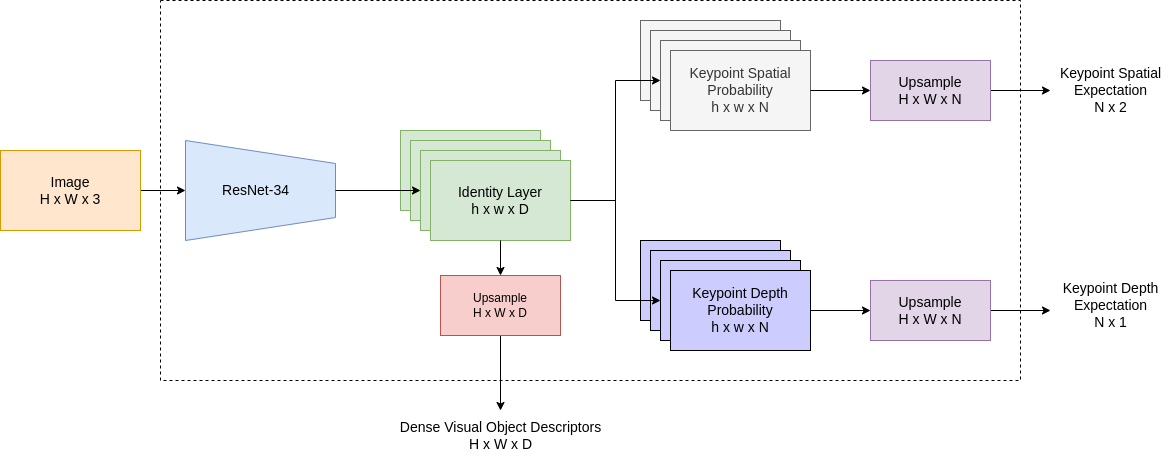
\includegraphics[scale=0.3]{images/arch.png}
    \caption{Illustration of novel DNN architecture designed to efficiently compute and seamlessly extract dense visual object descriptors.
        During inference we extract dense visual object descriptors directly from the network and ignore predicted spatial-depth expectation of the keypoints.}
    \label{fig:modified_dnn}
\end{figure}

\begin{figure}[htb]
    \centering
    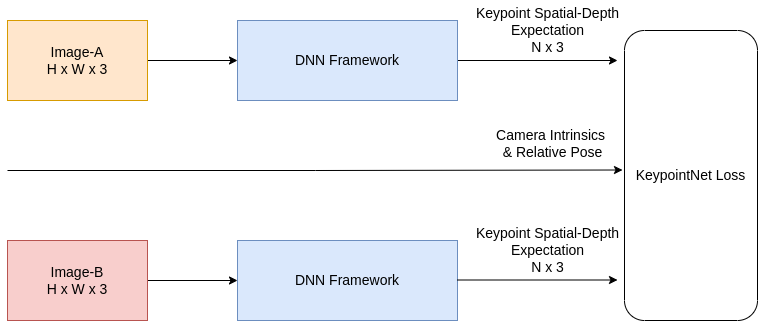
\includegraphics[scale=0.3]{images/twin.png}
    \caption{Depiction of twin DNN architecture's training strategy.}
    \label{fig:twin_architecture}
\end{figure}






\subsection{Loss Function Modifications}

For training, we directly adopt silhoutte consistency loss ($\mathcal{L}_{obj}$), variance loss ($\mathcal{L}_{var}$) and separation loss ($\mathcal{L}_{sep}$) functions from \cite{suwajanakorn2018discovery} to train the network on the keypoint prediction task.
However, we modify the multi-view consistent loss and relative pose estimation loss. In the case of multi-view consistency loss we
project the predicted spatial-depth expectation using camera intrinsics as follows:
\begin{equation}
    X_{cam} \in \mathbb{R}^{3 \times 1} = \mathcal{I}_{cam}^{-1}  \ [u, v, 1.0]^T \otimes d \text{ , where  } \ \mathcal{I}_{cam} \in \mathbb{R}^{3 \times 3} \text{ and }  u, v, d \in \mathbb{R}^+.
\end{equation}

Furthermore, we project the camera coordinates of the keypoints regressed on both images to the
world coordinates using camera transformation and compute Huber Loss~\cite{huber1992robust} represented as $\mathcal{H}$ in Equation~\ref{eqn:mvc} as multi-view consistency loss as follows:
\begin{equation}
    \label{eqn:mvc}
    \mathcal{L}_{mvc} \in \mathbb{R} = \mathcal{H}(\mathcal{T}_{C \rightarrow W}^A \hat{X}^A_{cam}, \mathcal{T}_{C \rightarrow W}^B \hat{X}^B_{cam}) \text{ , where  } \ \mathcal{T}_{C \rightarrow W} \in SE(3) \text{ and } \hat{X}_{cam}=[X_{cam}, 1.0]^T \in \mathbb{R}^{4 \times 1} ,
\end{equation}

this modification is geometrically more intuitive as all the keypoints projected from different camera viewpoints into world coordinates occupy the same value
addtionally, using Huber Loss creates smoother gradients to optimize the DNN compared to the original implementation of Euclidean distance.
In Equation~\ref{eqn:mvc} $SE(3) \in \mathbb{R}^{4 \times 4}$ is a ``Special Euclidean Group''~\cite{thurston2014three}.
We do not discard the relative transformation information to calculate the realative pose loss as suggested in \cite{suwajanakorn2018discovery}
and being influenced from \cite{zhao2020learning} we modified the relative pose loss as follows:
\begin{equation}
    \mathcal{L}_{pose} = \Vert log(\mathcal{T}_{truth}^{\dagger} \mathcal{T}_{pred}) \Vert \text{ , where  } \ log: SE(3) \rightarrow \mathfrak{se}(3) \text{ and } \mathcal{T}^{\dagger} = \begin{bmatrix}
        R^T & -R^T t \\
        0^T & 1
    \end{bmatrix} \in SE(3).
\end{equation}


\subsection{Controlled Dataset Engineering}

We have chosen the cap object for creating synthetic dataset as the cap mesh models are readily available in the ``Shapenet'' library~\cite{chang2015shapenet}
as it possess rich object information including textures.
Blenderproc~\cite{blenderproc} is used to generate the synthetic cap dataset by using of the 10 number of cap models from \cite{chang2015shapenet} library.
Futhermore, the caps are chosen such that each of them have distinct shapes, designs and colors.
For this controlled dataset, 100 random cameras are added in the environment with random poses capturing depth,
camera extrinsics information (referring to $\mathcal{T}_{C \rightarrow W}$ in Equation~\ref{eqn:mvc}) and object mask for each viewpoint for each cap model.
To make the training more robust such that networks are more object-centric, the images are additionally augmented with random backgrounds and noisy backgrounds
as depicted in Figure~\ref{fig:back_augmentations} in page~\pageref{fig:back_augmentations}
in addition to the color jitter and greyscale augmentations. For color jitter and greyscale augmentation we use available ``Torchvision''~\cite{marcel2010torchvision} library.


\begin{figure}[htb]
    \centering
    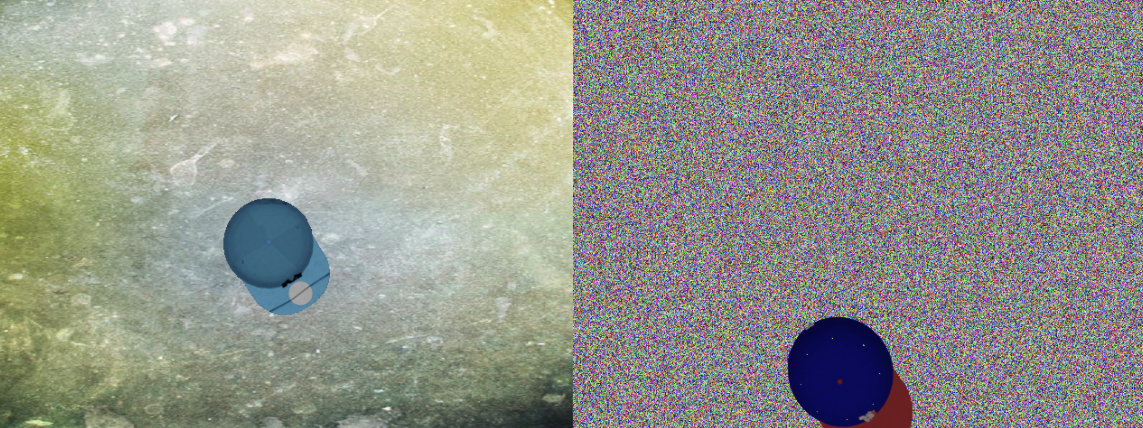
\includegraphics[scale=0.2]{images/back_augs.png}
    \caption{The image in the right illustrates the noisy background augmentation and the image in left depicts random background augmentation.}
    \label{fig:back_augmentations}

\end{figure}